\documentclass[11pt]{article}
\usepackage{fullpage}
\usepackage{graphicx}
\usepackage{float}
\usepackage{amsmath, amsfonts}
\usepackage[utf8]{inputenc}
\usepackage{tabu}

\begin{document}
\begin{center}
{{\Large \sc Computer Graphics}}
\end{center}
\rule{\textwidth}{1pt}
\begin{description}
\item[Student names and ids:] Andreas Jensenius (s093199) \& Jannick (s09) 
\item[Title :] Final project
\end{description}
\rule{\textwidth}{1pt}

Work distribution is equal. We worked together on all exercises, project and report and each contributed 50\%. 

\section{Exercise 1}
\subsection{Part 1}
\subsubsection{A}
The function \texttt{display} is the display function used by openGL, as defined by \texttt{glutDisplayFunc(display)}, and is called continuously. It defined which shaders to use, binds the VAO, draws the triangle and handles the swapping of buffers.\\

\noindent The function \texttt{reshape} handles the resizing of the window.\\

\noindent The function \texttt{loadBufferData} sets up the buffers and attaches the VAO.\\

\noindent The function \texttt{loadShader} sets up the shader and sets up the transfer of data to the shader.\\

\noindent The function \texttt{main} is the one which is run when executing the program. It sets up openGL/glut.

\subsubsection{B}
\begin{figure}[H]
\centering
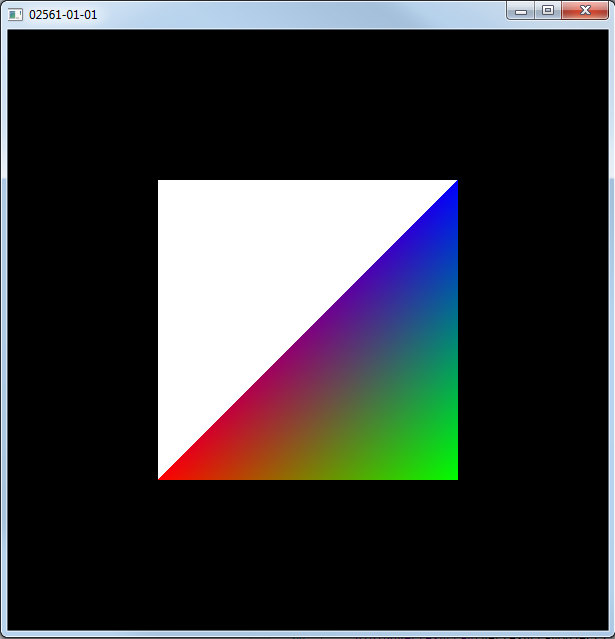
\includegraphics[width=0.5\linewidth]{images/e01p1b}
\label{fig:e01p1b}
\end{figure}

\subsection{Part 2}
\subsubsection{B}
\begin{figure}[H]
\centering
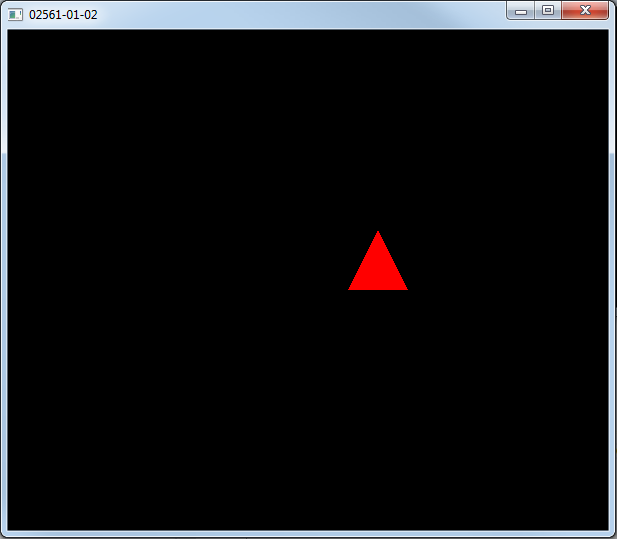
\includegraphics[width=0.5\linewidth]{images/e01p2b}
\label{fig:e01p2b}
\end{figure}

\subsubsection{C}
\begin{figure}[H]
	\centering
	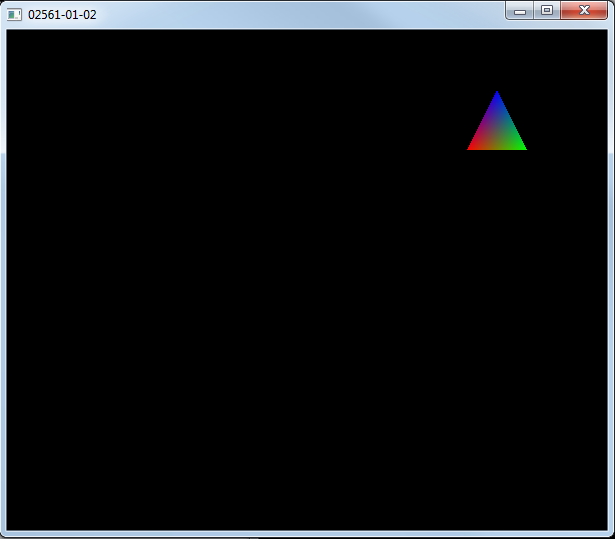
\includegraphics[width=0.5\linewidth]{images/e01p2c}
	\label{fig:e01p2c}
\end{figure}

\subsubsection{D}
\begin{figure}[H]
	\centering
	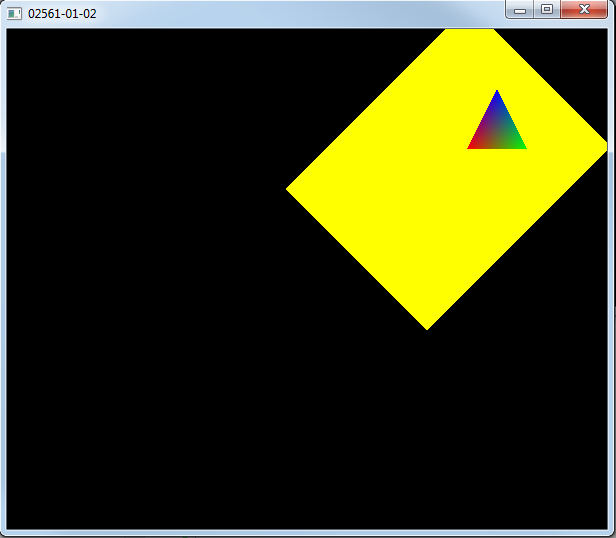
\includegraphics[width=0.5\linewidth]{images/e01p2d}
	\label{fig:e01p2d}
\end{figure}

\subsection{Part 3}
\subsubsection{A}
glDrawElements uses the given indices within to specify in which order the points should be used, instead of using them from 0 to end as glDrawArrays does.

\subsubsection{B}
$ GL_TRIANGLES $ simply forms triangles from three points. Given 6 points it would create 2 triangles.\\

\noindent $ GL_TRIANGLE_STRIP $ creates connected triangles, in which the two last points of the previous triangle are used as the two first point of the next triangle.\\

\noindent $ GL_TRIANGLE_FAN $ uses the first point given for every triangle it draws. Given 3 points it draws a triangle. For each new point given it creates adds a new connected triangle, using the newly added point, the first point given, and the previously added point.

\subsubsection{C}
\begin{figure}[H]
	\centering
	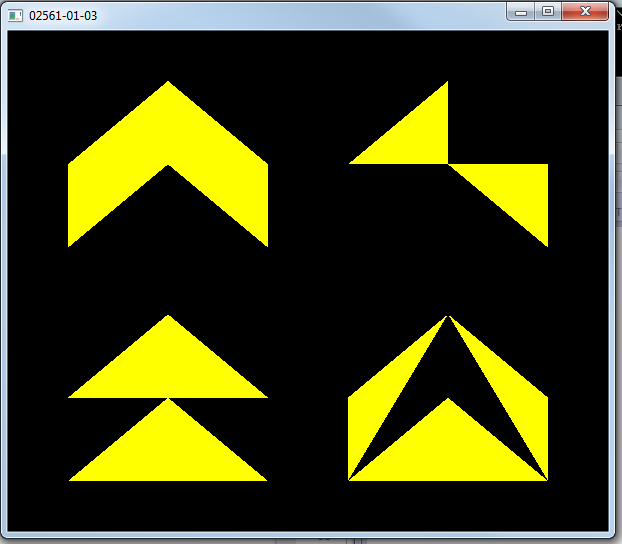
\includegraphics[width=0.5\linewidth]{images/e01p3c}
	\label{fig:e01p3c}
\end{figure}

\subsection{Part 4}
\begin{figure}[H]
	\centering
	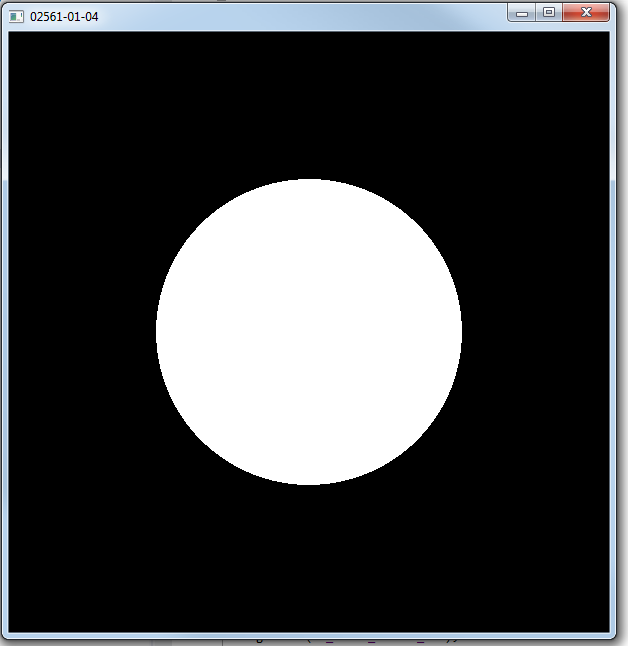
\includegraphics[width=0.5\linewidth]{images/e01p4}
	\label{fig:e01p4}
\end{figure}

\subsection{Part 5}
\begin{figure}[H]
	\centering
	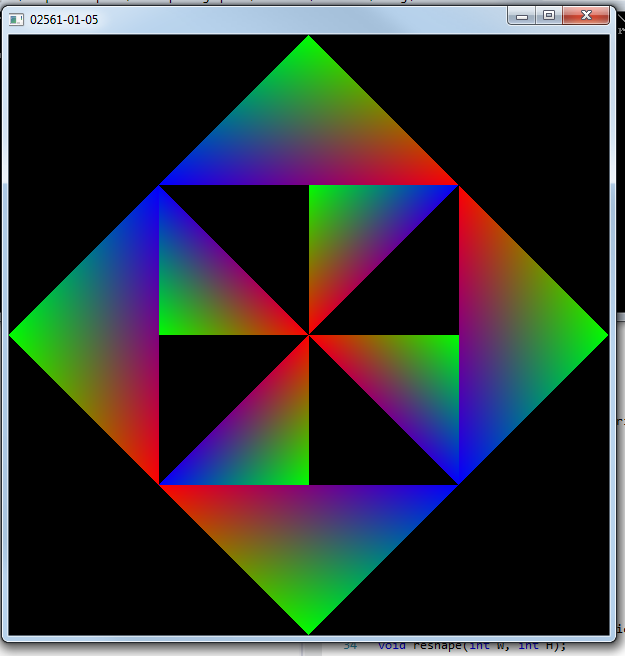
\includegraphics[width=0.5\linewidth]{images/e01p5}
	\label{fig:e01p5}
\end{figure}




\section{Exercise 2}
\subsection{Part 1}
The main difference between the two \texttt{display} functions is that this one defines "the camera" by creating the modelview.\\

\noindent The difference in the \texttt{vertex} struct is that the old struct handles both color and 2D position, whereas the one in exercise 2 handles position in 3D and not color. 

\subsection{Part 2}
\subsubsection{A}
\begin{figure}[H]
	\centering
	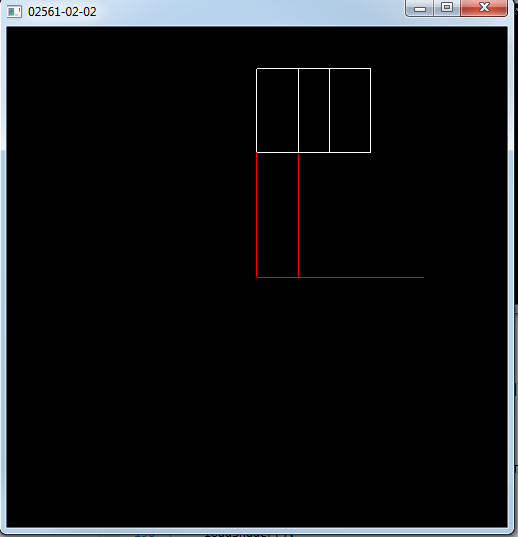
\includegraphics[width=0.5\linewidth]{images/e02p2a}
	\label{fig:e02p2a}
\end{figure}

\subsubsection{B}
Translate(0,3,0), Scale(2) and RotateY(30) was used.

\subsubsection{C}
First Translate, then Scale and finally RotateY.


\subsection{Part 3}
\subsubsection{A}
\begin{figure}[H]
	\centering
	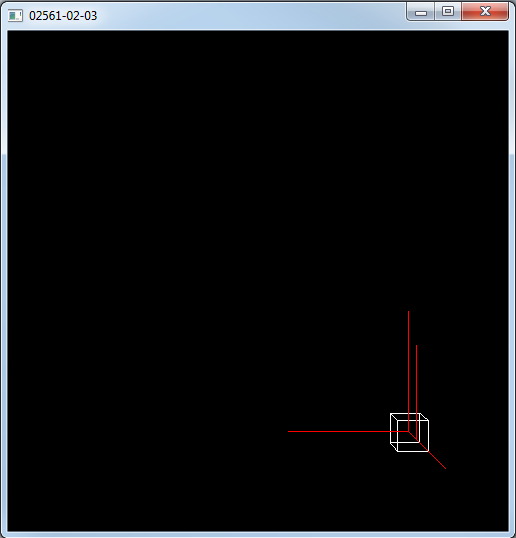
\includegraphics[width=0.5\linewidth]{images/e02p3a}
	\label{fig:e02p3a}
\end{figure}


\subsubsection{B}
\begin{figure}[H]
	\centering
	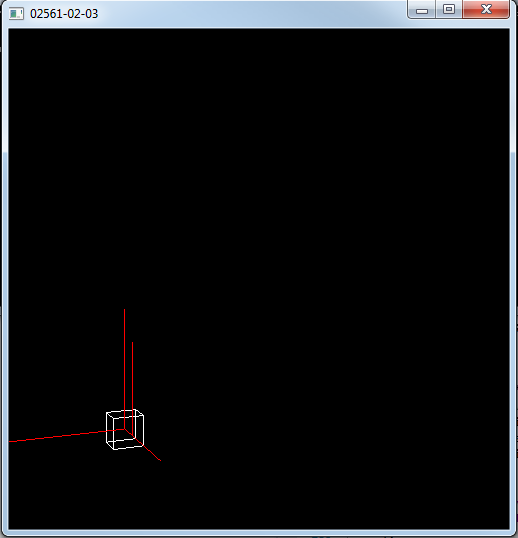
\includegraphics[width=0.5\linewidth]{images/e02p3b}
	\label{fig:e02p3b}
\end{figure}

\subsection{Part 4}
\begin{figure}[H]
	\centering
	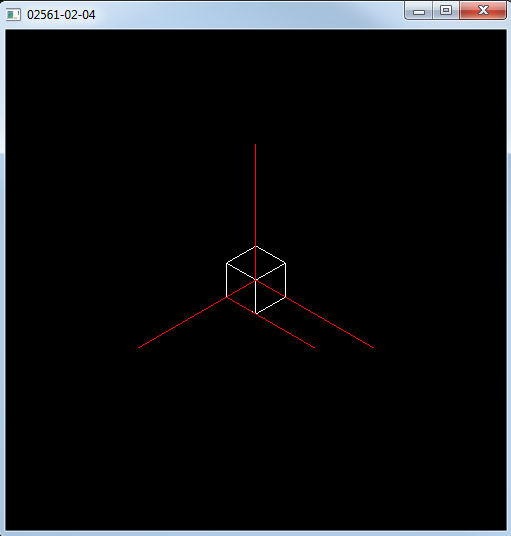
\includegraphics[width=0.5\linewidth]{images/e02p4}
	\label{fig:e02p4}
\end{figure}

\subsection{Part 5}
\subsubsection{key 2}
\begin{figure}[H]
	\centering
	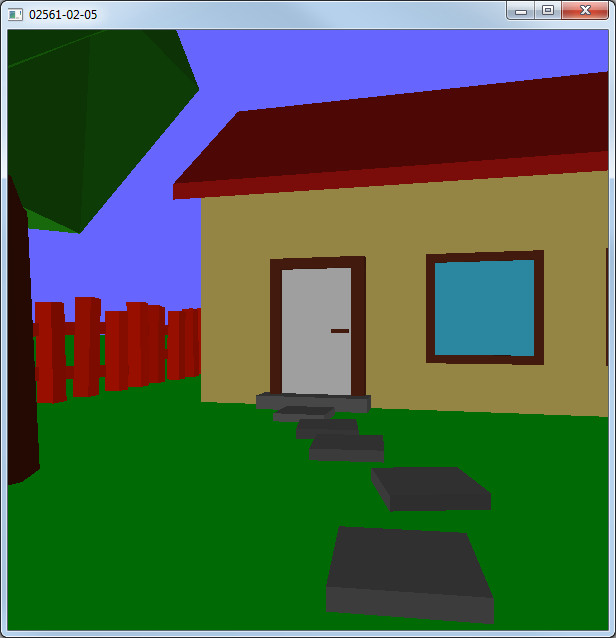
\includegraphics[width=0.5\linewidth]{images/e02p5key2}
	\label{fig:e02p5key2}
\end{figure}

\subsubsection{key 4}
\begin{figure}[H]
	\centering
	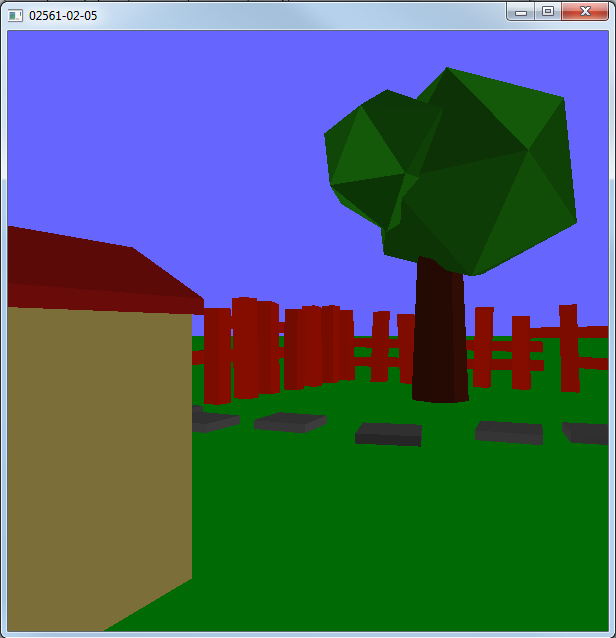
\includegraphics[width=0.5\linewidth]{images/e02p5key4}
	\label{fig:e02p5key4}
\end{figure}

\subsubsection{key 6}
\begin{figure}[H]
	\centering
	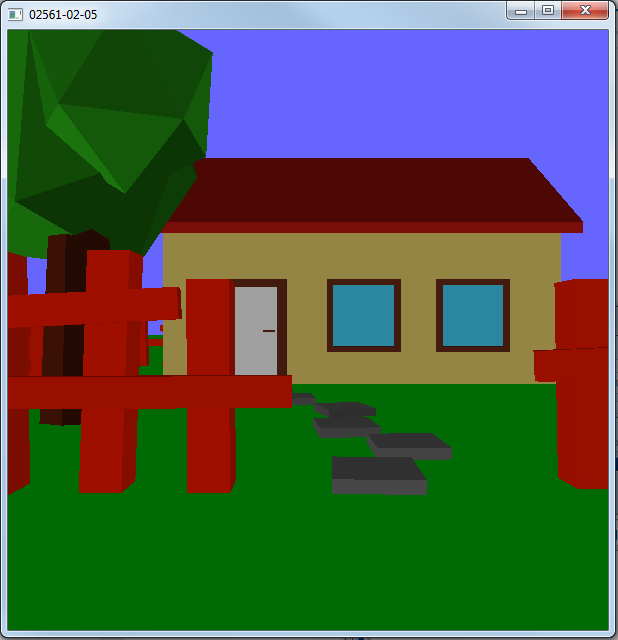
\includegraphics[width=0.5\linewidth]{images/e02p5key6}
	\label{fig:e02p5key6}
\end{figure}


\subsection{Part 6}
\textbf{!!!! INDSÆT FORKLARING HER !!!!}



\section{Exercise 3}
\subsection{Part 1}
\begin{figure}[H]
	\centering
	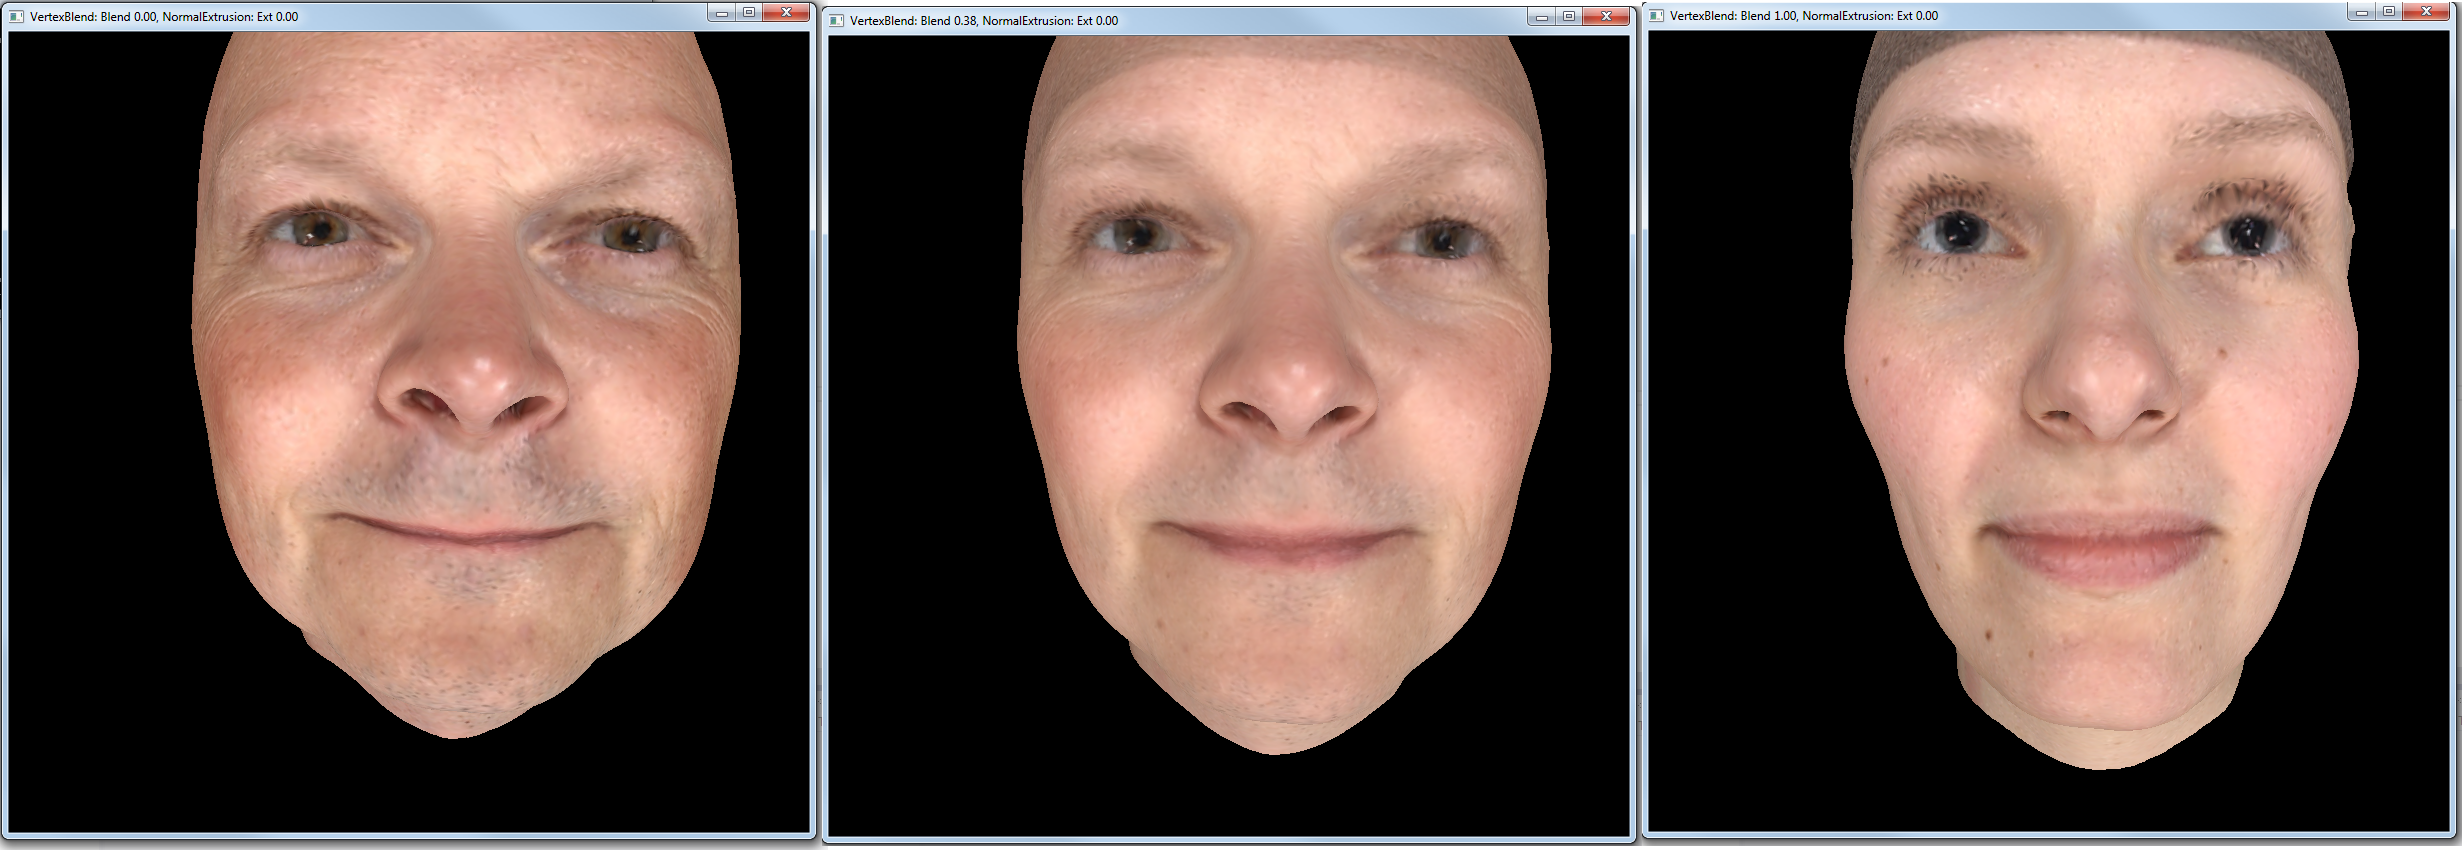
\includegraphics[width=0.5\linewidth]{images/e03p1}
	\label{fig:e03p1}
\end{figure}


\subsection{Part 2}
\begin{figure}[H]
	\centering
	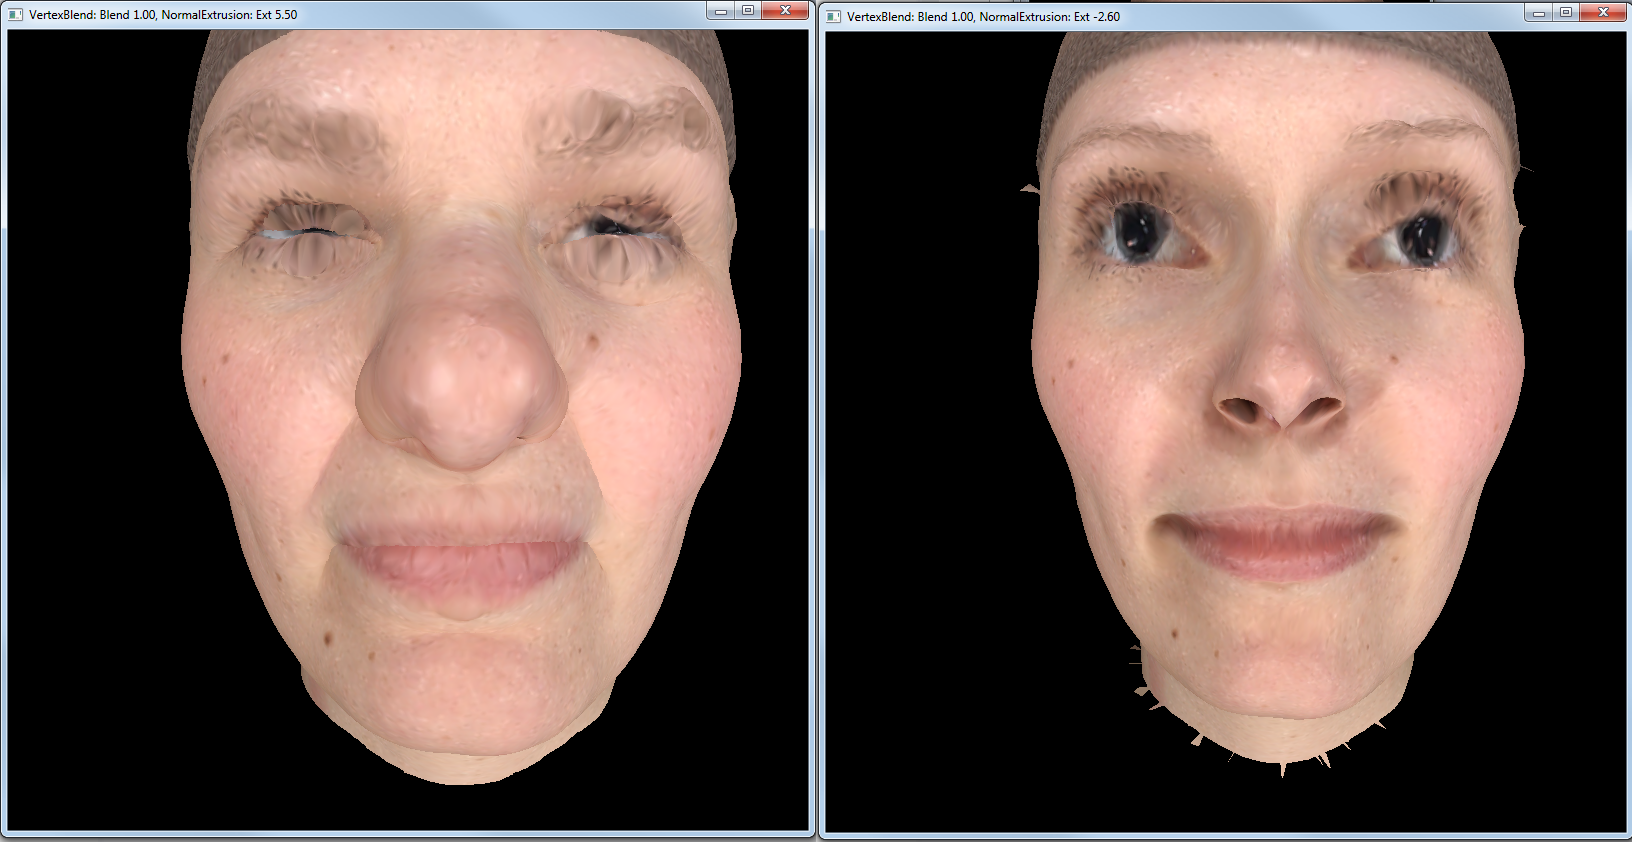
\includegraphics[width=0.5\linewidth]{images/e03p2}
	\label{fig:e03p2}
\end{figure}


\subsection{Part 3}
\textbf{!!!! INDSÆT FORKLARING HER !!!!}


\section{Exercise 4}
\subsection{Part 1}
\begin{figure}[H]
	\centering
	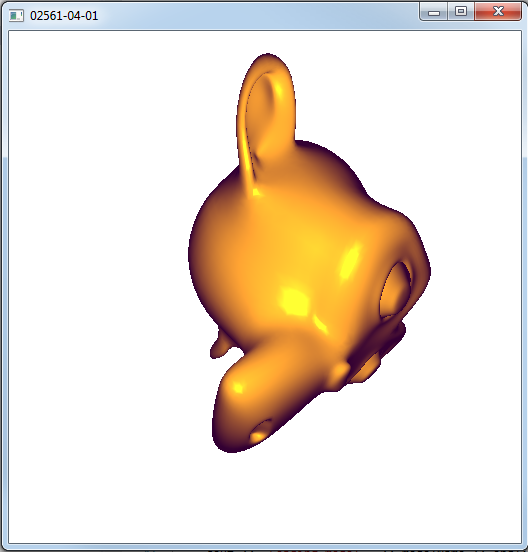
\includegraphics[width=0.5\linewidth]{images/e04p1}
	\label{fig:e04p1}
\end{figure}

\subsection{Part 2}
First is point light, second is directional.
\begin{figure}[H]
	\centering
	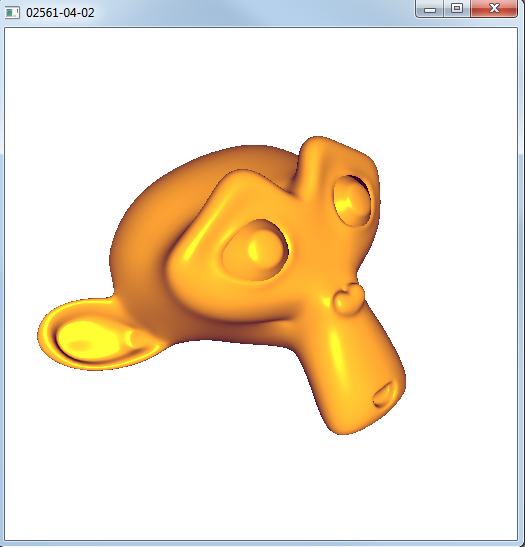
\includegraphics[width=0.5\linewidth]{images/e04p2point}
	\label{fig:e04p2point}
\end{figure}
\begin{figure}[H]
	\centering
	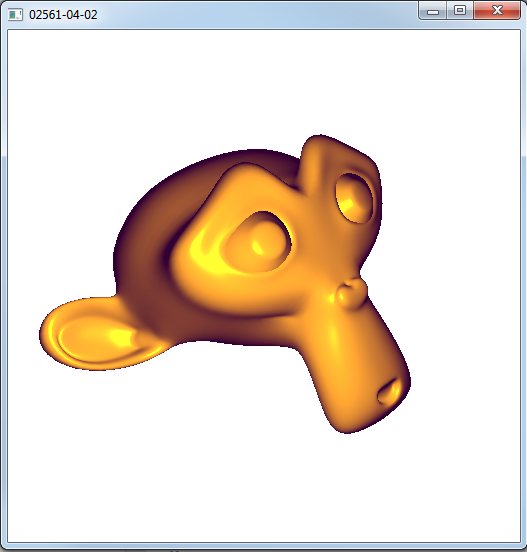
\includegraphics[width=0.5\linewidth]{images/e04p2directional}
	\label{fig:e04p2directional}
\end{figure}

\subsection{Part 3}
\subsubsection{A}
\textbf{!!!! INDSÆT FORKLARING HER !!!!}


\subsubsection{B}
Gouraud shading is applied on a vertex level, while Phong shading is applied on a per-fragment level. Gourad is cheaper but makes the model look more rough, and phong is more expensive but makes it look more smooth.


\subsubsection{C}
Using point light, the light originates from a single point with a given direction, while directional lighting does not have a specific origin. In directional light all the light rays are parallel, while using point light the light rays starts from the same origin and spread out.


\subsubsection{D}
Yes.


\subsubsection{E}
It simply removes the specular component.


\subsubsection{F}
It makes it look more shiny, like polished metal, by increasing the intensity of specular lighting.


\subsubsection{G}
We made no simplifications.


\subsubsection{H}
It is used to convert to normal vector into eye space. You obtain the normal matrix by taking the transpose, inverse of the modelview matrix.


\subsubsection{I}
Eye-space.

\subsection{Part 4}
\begin{figure}[H]
	\centering
	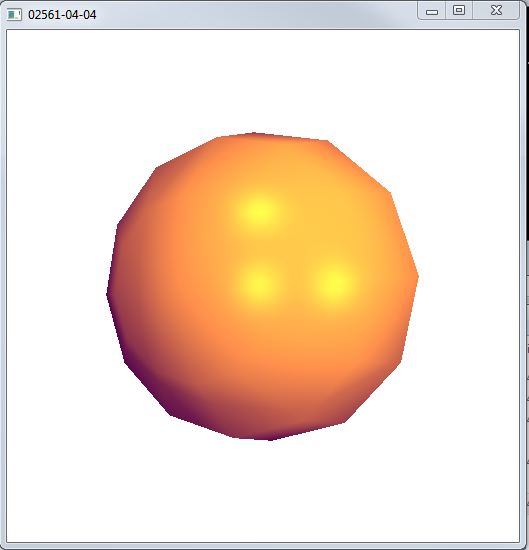
\includegraphics[width=0.5\linewidth]{images/e04p4}
	\label{fig:e04p4}
\end{figure}

\section{5}
\subsection{Part 1}
Pick select which object to draw once you click outside the colored boxes.

\subsection{Part 2}
When the user clicks on a square the uniform variable colorUniform is set and the frameBufferObject i bound. renderScene(true) generates the color and stores, and we then retrieve it in getId decoded from a color. The value of the selected index on the board is update to one of the three possible colors, and we ask to have the display function run again, so that renderScene(false) can draw our changes

\subsection{Part 3}
\subsubsection{A}
\begin{figure}[H]
	\centering
	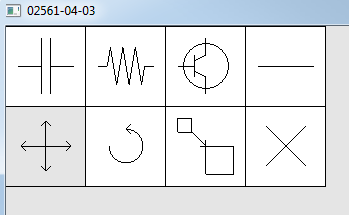
\includegraphics[width=0.5\linewidth]{images/e05p3a}
	\label{fig:e05p3a}
\end{figure}

\subsubsection{B}
When doing screenshots, the cursor is not captured in the image so it is not shown on the image below.
\begin{figure}[H]
	\centering
	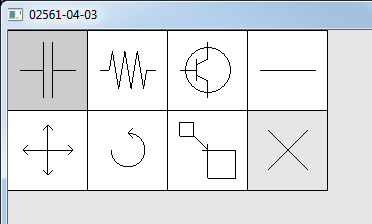
\includegraphics[width=0.5\linewidth]{images/e05p3b}
	\label{fig:e05p3b}
\end{figure}

\subsubsection{C}
\begin{figure}[H]
	\centering
	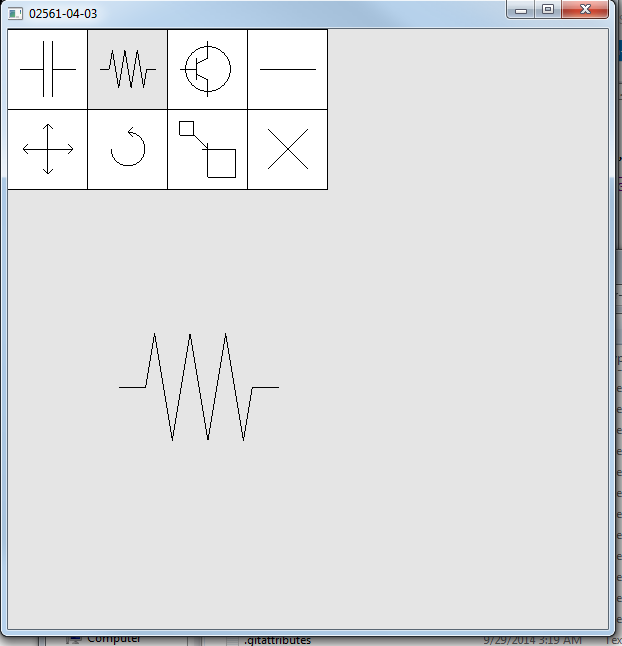
\includegraphics[width=0.5\linewidth]{images/e05p3c}
	\label{fig:e05p3c}
\end{figure}

\subsubsection{D}
\begin{figure}[H]
	\centering
	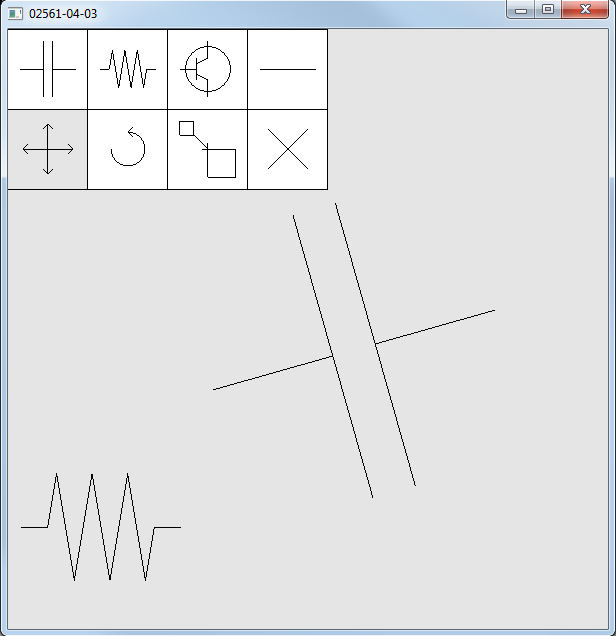
\includegraphics[width=0.5\linewidth]{images/e05p3d}
	\label{fig:e05p3d}
\end{figure}

\subsubsection{E}
\begin{figure}[H]
	\centering
	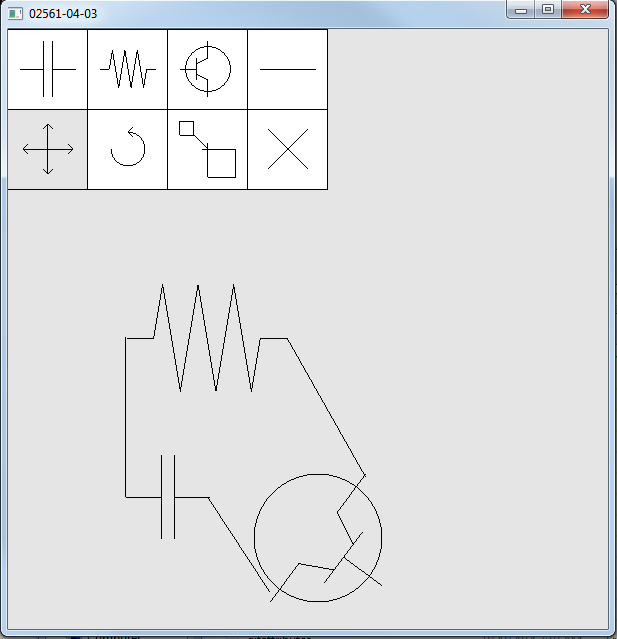
\includegraphics[width=0.5\linewidth]{images/e05p3f}
	\label{fig:e05p3f}
\end{figure}



\section{Exercise 6}
\subsection{Part 1}
\subsubsection{A}
\textbf{!!!! INDSÆT JANNICK TEGNING !!!!}

\subsubsection{B}
The small green object is rotated along the y-axis which makes it face away from the eye point. Face culling then removes it.

\subsubsection{C}
OpenGL decides what the orientation is, by looking at the direction of a surface's normal vector.


\subsection{Part 2}
\begin{figure}[H]
	\centering
	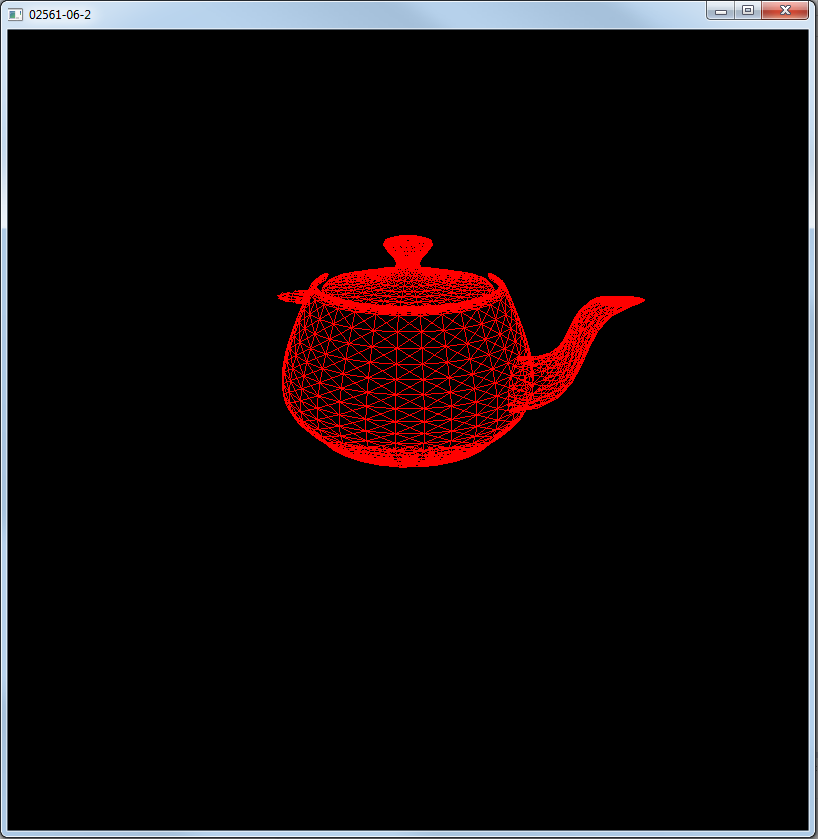
\includegraphics[width=0.5\linewidth]{images/e06p2}
	\label{fig:e06p2}
\end{figure}


\subsection{Part 3}
\begin{figure}[H]
	\centering
	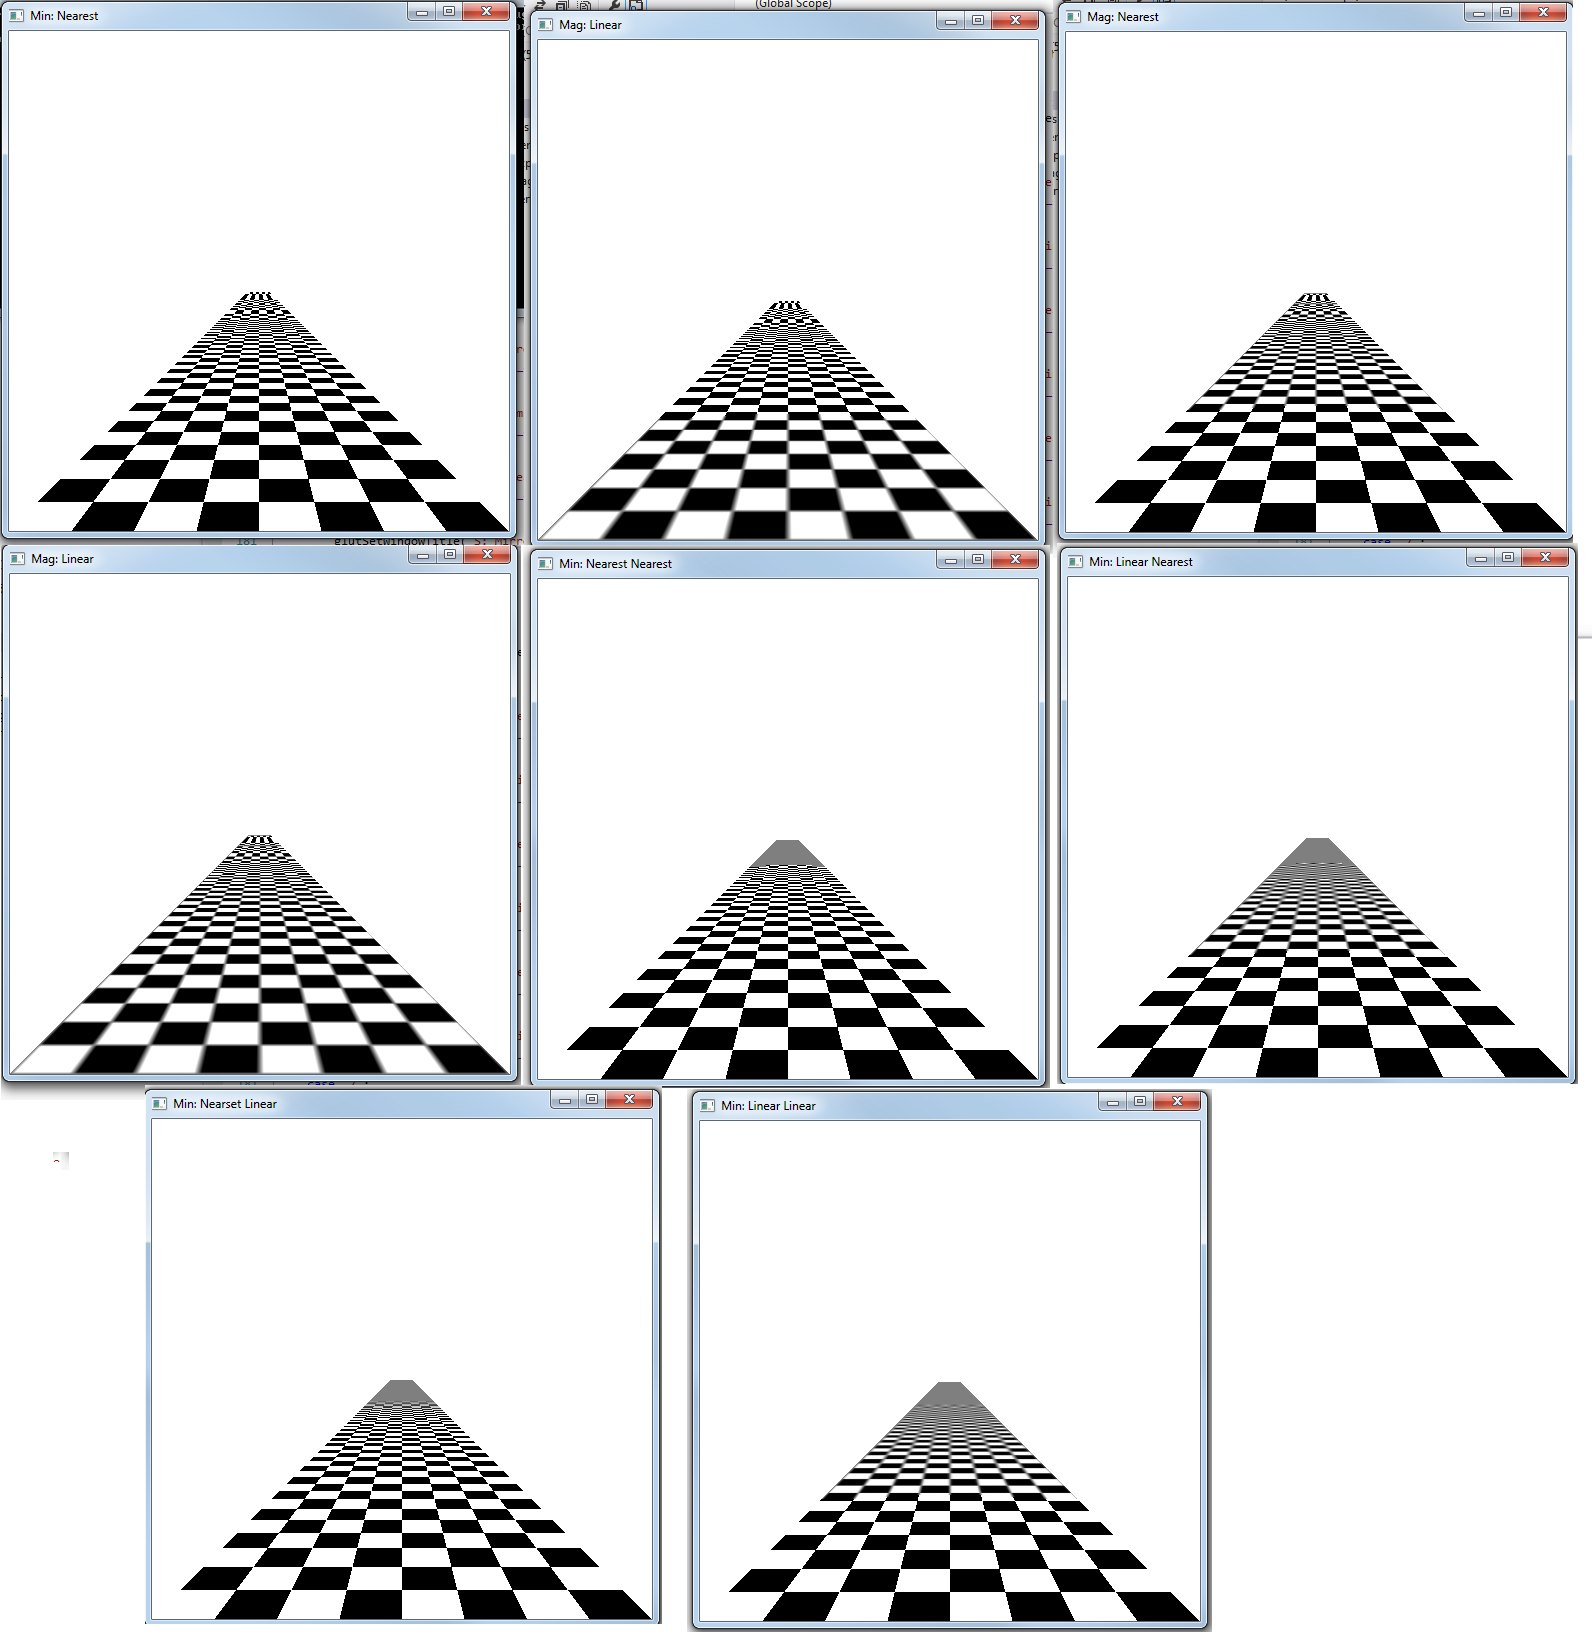
\includegraphics[width=0.5\linewidth]{images/e06p3}
	\label{fig:e06p3}
\end{figure}

\subsection{Part 4}
\begin{figure}[H]
	\centering
	\includegraphics[width=0.5\linewidth]{images/e06p4}
	\label{fig:e06p4}
\end{figure}

\subsection{Part 5}
\begin{figure}[H]
	\centering
	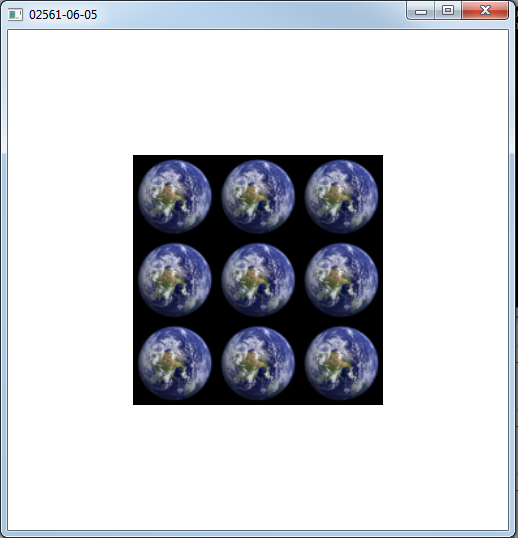
\includegraphics[width=0.5\linewidth]{images/e06p5}
	\label{fig:e06p5}
\end{figure}










\end{document}